\section{Worked example of single player dynamics}\label{sec:single-player-example}

In this section we propose a dynamic system for a very simple network and show that it preserves as an invariant equilibrium traffic flow with respect to a (changing) control parameter $y$.

\subsection{Notation}

We will consider the following network.

\begin{figure}[!ht]
    \centering
    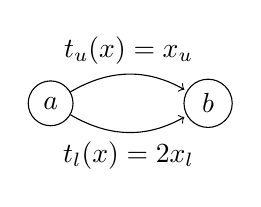
\begin{tikzpicture}[vertex/.style={circle, draw}]
        \node[style=vertex] (a) at (0, 0)  {$a$};
        \node[style=vertex] (b) at (2, 0)  {$b$};
        
        \draw[every loop]
            (a) edge [bend left] node[above] {$t_{u}(x)=x_{u}$} (b)
            (a) edge [bend right] node[below] {$t_{l}(x)=2x_l$} (b)
        ;
    \end{tikzpicture}
    \caption{An example network. Each link is labeled with the link cost function.}
    \label{fig:example-netowkr}
\end{figure}

In this example network there are two nodes, $a$ and $b$, and two links, $u$ and $l$. 
Because of this special structure, the links are also the two paths, so link and path will be used interchangeably.
The only origin destination pair is $(a, b)$.
The demand from $a$ to $b$ is given by $q=6$.
The volume on link $l$ is given by $x_l$ and on link $u$ by $x_u$.
The vector of link flow is given by $x=[x_u, x_l]$.
The vector-valued link cost function is given by $t(x) = [t_u(x), t_l(x)]$.

The feasibility constraints are given by \eqref{eqn:appendix:feasibility}.

\begin{subequations}
\begin{align}
    x_u &\geq 0\\
    x_l &\geq 0\\
    x_l + x_u &= q
\end{align}\label{eqn:appendix:feasibility}
\end{subequations}

The feasible link flows are given by the set $\Omega = \{ (x_u, x_l) \mid x_u, x_l \geq 0, x_u +x_l = q\}$.

\subsection{Equilibrium as a dynamical system}

The dynamical system we are interested in is given by 

\begin{align}
    x' &= \Pi_{\Omega}(x, -t(x))\label{eqn:appendix:project-dynamical-system}
\end{align}

\begin{remark}[Expressible in dL]
\label{remark:dl-expression}
The system given by \eqref{eqn:appendix:project-dynamical-system} is expressible in dL extended with $\min$ and $\max$ as in KeYmeara X.
\end{remark}

In general we should not expect projection onto a simplex to be expressible in first order arithmetic.
However, the feasible region $\Omega$ is the straight line connecting $(0, q)$ and $(q, 0)$. 
The normal to this line is given by $(1, 1)$, so we simply follow this vector until the constraint is met.
Explicitly, this distance is given by $\alpha = \frac{q-x_1-x_2}{2}$.
This will ensure that the demand constraint is met, but not necessarily the non-zero constraints. 
In full, the projected values $\hat{x}_u = P(x_u) = \min(\max(0, x_u+\alpha), q)$ and $\hat{x}_l = P(x_l) = \min(\max(0, x_l+\alpha), q)$.

\begin{remark}[Feasibility invariant]
The system given by \eqref{eqn:appendix:project-dynamical-system} preserves feasibility as an invariant.
\end{remark}

The projection operator implicitly enforces the feasibility of link flows.\\

\subsection{Equilibrium with respect to a control variable}

Suppose a traffic controller is able to influence the link cost function, for example, by applying a toll to one or more links.
Concretely consider the following network, modified slightly from \cref{fig:example-netowkr}.
The equilibrium condition remains the same: 
\begin{align}
    0&= \Pi_{\Omega}(x, -t(y, x))\label{eqn:appendex:equilibrium-wrt-y}
\end{align}
However, because the link cost now depends on $y$, link flows that satisfy the condition are called equilibria with respect to $y$.

\begin{figure}[!ht]
    \centering
    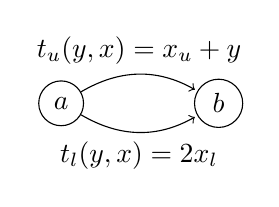
\begin{tikzpicture}[vertex/.style={circle, draw}]
        \node[style=vertex] (a) at (0, 0)  {$a$};
        \node[style=vertex] (b) at (2, 0)  {$b$};
        
        \draw[every loop]
            (a) edge [bend left] node[above] {$t_{u}(y, x)=x_{u} + y$} (b)
            (a) edge [bend right] node[below] {$t_{l}(y, x)=2x_l$} (b)
        ;
    \end{tikzpicture}
    \caption{An example network. Each link is labeled with the link cost function.}
    \label{fig:example-netowkr}
\end{figure}

The link cost functions are now functions of the link flow $x$ and the control variable.
We assume that $y$ is constrained to be non-negative.

In the case where $y$ is fixed, the problem reduces to the previous section, with a slightly different link cost function.
We are interested in the case where $y$ is changing.
Concretely, we would like to define dynamics for $x$ such that equilibrium with respect to the control variable $y$ is an invariant of the dynamics\textemdash even as the value of $y$ is continuously changing.

To achieve this, we modify the dynamics slightly from the previous section.

\begin{subequations}
\begin{align}
    x' &= \Pi_{\Omega}\left(x, -\left(t(x) + \gamma h \right)\right)\\
    y' &= h \\
       &\& y \geq 0
\end{align}\label{eqn:appendix:single-player-dynamics}
\end{subequations}

Where we take $h$ a positive constant and $\gamma$ will be specified below.

We can generate an intuition for this system from inspecting the time derivative of the link cost.
\begin{align}
    t' &= \frac{\partial t}{\partial x} x' + \frac{\partial t}{\partial y}y'
\end{align}

In this system the link cost is changing not only in response to how the link flow is changing but how the control parameter is changing.
The additional term in $x'$ adjusts the direction of flow change to cancel the direction in which the link cost is changing as a result of the control.
In effect, this ensures that the flow is always changing in the direction of equilibrium which is now moving as $y$ changes and that the invariant remains the equilibrium condition with respect to $y$: $0= \Pi_{\Omega}(x, -t(y, x))$.

\begin{theorem}[Equilibrium Invariant]
    The equilibrium condition with respect to $y$ given by \eqref{eqn:appendex:equilibrium-wrt-y} is invariant under the system given by \eqref{eqn:appendix:single-player-dynamics}. 
\end{theorem}

\begin{proof}
    To prove \eqref{eqn:appendex:equilibrium-wrt-y} invariant under the dynamics given by \eqref{eqn:appendix:single-player-dynamics} it suffices to show that 
    \begin{align}
        \left(\Pi_{\Omega}(x, -t(y, x))^T\Pi_{\Omega}(x, -t(y, x))\right)' &\leq 0\label{eqn:eq-inv}
        \intertext{This is equivalent to the sum of the square of each component. From \cref{remark:dl-expression}, the projection can be written using first order arithmetic. Here we denote $\min(q, \max(0, \cdot))$ by $|_0^q\cdot$}
        \Pi_{\Omega}(x, -t(y, x)) &= -(\min(q, \max(0, \Phi_l)), \min(q, \max(0, \Phi_u)))\\
        \intertext{where $\Phi_l, \Phi_u$ are defined,}
        \Phi_l &= x_u - \sfrac{1}{2}(x_u - t_u - x_l - t_l) -\sfrac{1}{2}q\\
               &= \sfrac{1}{2}(t_u - t_l)\\
        \Phi_u &= x_l + \sfrac{1}{2}(x_u - t_u - x_l - t_l) -\sfrac{1}{2}q\\
               &= -\sfrac{1}{2}(t_u - t_l)\\
        \intertext{To simply we use the fact that $x_l+x_u = q$ is an invariant by construction. Expressing \eqref{eqn:eq-inv} in terms of $\Phi$,}
        ((|_0^q\Phi_l)^2 + (|_0^q\Phi_u)^2)' &\leq 0
        \intertext{Although the $|_0^q$ operator is not differentiable at $0$ or $q$, it does have well-defined sub- and super-differentials. Define $\mathbb{I}_P(x)$ as an indicator function for term $x$ and predicate $P$ which is 1 whenever $P(x)$ is true and 0 otherwise. Denote the set of sub-differentials of a function $f$ by $D\ f$. In particular,}
        \mathbb{I}_{0\leq f \leq q} &\in D\ |_0^q
        \intertext{So it follows (and analogously for $\Phi_u$),}
        -2(|_0^q\Phi_l)\mathbb{I}_{0\leq \Phi_l \leq q}(\Phi_l)\Phi_l' &\in D\ (|_0^q\Phi_l)^2
        \intertext{Because of the presence of the indicator, the only remaining $|_0^q$ may be dropped. This is so because $|_0^q\Phi_l$ evaluates to $\Phi_l$ whenever $\Phi_l \in [0, q]$. Outside this interval $|_0^q \Phi_l \neq \Phi_l$. However, the indicator function is $0$ everywhere \textit{except} where $\Phi_l \in [0, q]$. Therefore all terms on which the indicator is 0 drop and we are left with only those for which the indicator evaluates to 1. Concretely it now suffices to show,}
        -2\Phi_l\Phi_l' - 2\Phi_u\Phi_u' &\leq 0
        \intertext{Before moving forward a few useful simplifications. First, applying the same tricks to $x_l'$, $x_u'$ in \eqref{eqn:appendix:single-player-dynamics}, the adjustment can be extracted from the expression,}
        x'_u &= \Phi_1 - \sfrac{1}{2}(\gamma_u-\gamma_l)h\\
        x'_l &= \Phi_2 + \sfrac{1}{2}(\gamma_u-\gamma_l)h\\
        \intertext{Additionally, $t_u'$ and $t_l'$ are readily computed,}
        t'_u &= x'_u + y'\\
        t'_l &= 2x'_l\\
        \intertext{It follows that,}
        \Phi_l' &= \sfrac{1}{2}(t'_u - t'_l)\\
        -2\Phi_l\Phi_l' &= -2 (\sfrac{1}{2})(t_u - t_l)(\sfrac{1}{2})(\sfrac{3}{2}(t_u-t_l) - (\sfrac{3}{2})(\gamma_u - \gamma_l)h + h)\\
        \intertext{Taking $\gamma = (\frac{2}{3}, 0)$ cancels the $h$ term yielding,}
        -2\Phi_l\Phi_l' &= -(\sfrac{3}{4})(t_u - t_l)^2 \leq 0\\
        \intertext{Additionally, since $\Phi_u = -\Phi_l$,}
        -2\Phi_l\Phi_l' - 2\Phi_u\Phi_u' &=  -2\Phi_l\Phi_l' - 2(-\Phi_l)(-\Phi_l)'\\
            &= -4\Phi_l\Phi_l' \leq 0\\
    \end{align}
    
    The theorem is proved.
\end{proof}